\section{Representación de soluciones activas basada en llaves aleatorias}
La representación propuesta se basa en asignar a cada operación una número real entre 0 y 1 el cual sirve para definir un orden entre operaciones en una misma máquina mediante un proceso de decodificación un planteamiento similar puede encontrarse en \cite{bean1994genetic,norman1996random,Ponsich2013}.

Para decodificar la solución a partir de las llaves se utiliza el algoritmo de Giffler \& Thompson \cite{Giffler1960} con el cual se generan soluciones activas.\\ 

Una consecuencia importante de este cambio en la representación es que el espacio de búsqueda se reduce a solo las soluciones activas y como se sabe que las planificaciones óptimas son un subconjunto de estas, esta representación puede representar cualquier solución óptima. 
\\

Un punto negativo es que esta representación es n a 1 porque solo importa el tamaño relativo de las llaves que compiten entre sí, es decir que diferentes valores de llaves pueden llevarnos a la misma solución. En principio no parece un problema muy grave aunque sería más eficiente tener una representación 1 a 1.

A continuación se presenta el algoritmo para construir planificaciones activas de llaves numéricas.

\subsection{Algoritmo de Giffler \& Thompson}
Para explicar el algoritmo de Giffler \& Thompson se adoptan las siguientes notaciones:
\begin{itemize}
    \item $O_i$ la operación $i$.
    \item $M(O_i)$ la máquina en la que debe procesarse la operación $O_i$.
    \item $t_f(O_i)$ el tiempo en que se terminaría de procesar la operación $O_i$ si se planifica en este paso.
    \item $t_i(O_i)$ el tiempo en que se comenzaría a procesar la operación $O_i$ si se planifica en este paso.
    \item $k(O_i)\in [0,1]$ el valor de la llave asignada a $O_i$.
\end{itemize}

El primer paso es marcar como planificable la primera operación de cada trabajo. Posteriormente se identifica la operación $O_{min}$ con el menor tiempo de finalización si se planificase en este paso y la máquina $M^*=M(O_{min})$ en la cuál debe procesarse. Se toma el tiempo de finalización $t^*_f = t_f(O_{min})$ para escoger alguna de las operaciones planificables en $m^*$ cuyo tiempo de inicio sea menor a $t^*_f$, se actualizan las operaciones planificables y este proceso se repite hasta completar la planificación. El algoritmo es el siguiente:\\ 

\begin{algorithm}[H]
 \KwData{Instancia del JSP}
 \KwResult{Planificación activa}
 Inicializar el conjunto de operaciones planificables $\Omega$\;
 \While{$\Omega$ no vacío}{
    Determinar la operación con el menor tiempo potencial de finalización $O_{min}=\arg\min_{O\in\Omega} \,\,t_f(O)$ \;
    Determinar el tiempo de finalización $t^*_f$ y la máquina $M^*$ en que se procesa $O_{min}$\;
    Identificar el conjunto $C\subset\Omega$ de operaciones que cumplen $t_i(O) < t^*_f$ y $M(O)=M^*$\;
    Escoger la operación $O^*\in C$ que tenga asignada la llave de mayor valor\;
    Asignar tiempo de inicio y fin a $O^*$\;
    Actualizar $\Omega$ eliminando a $O^*$ y agregando a su sucesora si existe\;
 }
    \label{alg:GT}
    \caption{Algoritmo de Giffler \& Thompson}
\end{algorithm}
\subsubsection*{Ejemplo}
Como ejemplo ilustrativo se muestran los primeros pasos para construir la planificación mostrada en la figura \ref{fig:gantt} asociada a la instancia de ejemplo mostrada en la tabla \ref{tab:inst}.\\

Para recuperar la planificación previamente mostrada se asignan las llaves de la siguiente manera: \[k(O_{00})=k(O_{01})=k(O_{02})=1\]  \[k(O_{10})=k(O_{11})=k(O_{12})=0\]
\begin{itemize}
    \item Se inicializa $\Omega$ agregando las operaciones iniciales de cada trabajo, es decir:

\[\Omega = \{O_{10},O_{00}\}\]

     \item Se identifica a la operación que acabaría primero si se planifica ya, en este caso es $O_{10}$ que se debe procesar en la máquina $M_0$. 

     \item Se identifican las operaciones que podrían comenzar a procesarse antes del tiempo potencial de finalización de $O_{10}$. En este caso solo $O_{00}$ y  $O_{10}$ cumplen las condiciones.

Como $k(O_{00})>k(O_{10})$ se planifica $O_{00}$ se le asignan $0$ y $54$ como tiempos inicial y final.

     \item Se actualiza $\Omega$ removiendo a la operación planificada y agregando a su sucesora $O_{02}$.

\[\Omega\leftarrow \{O_{10},O_{02}\}\]
\end{itemize}
Este proceso continua de acuerdo al algoritmo \ref{alg:GT} hasta que todas las operaciones se encuentren planificadas.\\ 

\subsection{Construcción de soluciones activas a partir de no activas}

Hasta ahora se ha considerado que la asignación de las llaves a las operaciones se hace de manera aleatoria. Esta asignación también puede hacerse tomando como base una solución previamente dada que no necesariamente tiene que ser activa. 

Como se vio en el modelo de grafo disyuntivo construir una planificación consiste en elegir direcciones de aristas disyuntivas. Esto al final genera un orden para las operaciones en cada máquina i.e. una permutación. Para hallar la representación de alguna de estas soluciones en el esquema propuesto se toma esta permutación de las operaciones para cada máquina y se le asigna a cada una una prioridad decreciente acuerdo a su posición en la permutación.
\[k(O_i)>k(O_{i+1})\]
\[\text{donde }O_i\text{ es la operación número $i$ en procesarse}\]

Esta asignación nos asegura que se mantenga el orden de muchas operaciones pero convierte a la solución en activa. A continuación se muestra un ejemplo ilustrativo

\subsubsection*{Ejemplo}
Consideremos la instancia del JSP mostrada en la siguiente tabla:
\begin{table}[H]
\centering
\begin{tabular}{@{}llll@{}}
Trabajo & \multicolumn{3}{l}{\begin{tabular}[c]{@{}l@{}}Secuencia de procesamiento \\ (máquina, tiempo)\end{tabular}} \\ \midrule
0 & 1, 37 & 0, 13 & 2, 35\\ \midrule
1 & 0, 8 & 1, 4 & 2, 9 \\\hline                         
2 & 1, 34 & 2, 72 & 0, 96 \\\hline                         
3 & 1, 63 & 0, 77 & 2, 24 \\\hline                         
\end{tabular}
\caption{Instancia 3 maquinas y 4 trabajos}
\label{tab:instactive}
\end{table}

La siguiente figura muestra un diagrama de gantt para una posible planificación.

\begin{figure}[H]
     \centering
     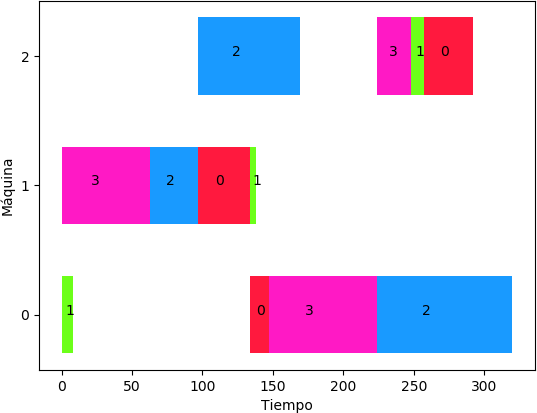
\includegraphics[scale=.7]{Imagenes/ganttnonactivepr.png}
     \caption{Planificación posible para la instancia en \ref{tab:instactive}. }
     \label{fig:nonactivepr}
\end{figure}
A partir de la planificación mostrada podemos asignar las prioridades del modo previamente dicho con lo que después de construir la planificación a partir de estas prioridades obtenemos la planificación que se muestra en la siguiente figura.
\begin{figure}[H]
     \centering
     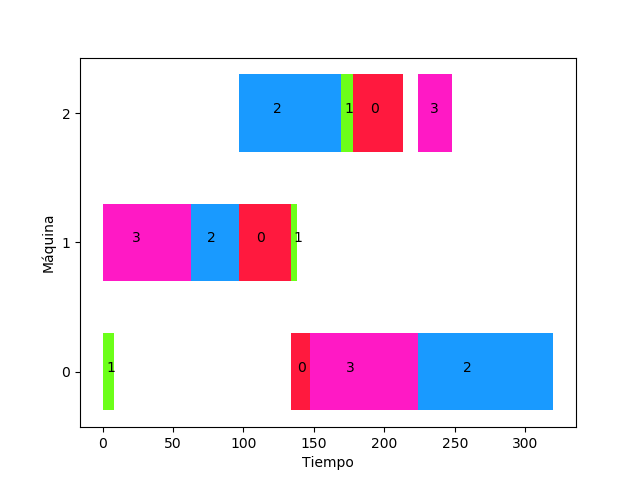
\includegraphics[scale=.7]{Imagenes/ganttactivepr.png}
     \label{fig:activepr}
     \caption{Planificación activa reconstruida a partir de la mostrada en \ref{fig:nonactivepr}}
\end{figure}

Podemos notar como dos operaciones cambian de lugar de modo que se planifican antes sin aumentar el tiempo de inicio de otras.

Una característica importante de esta representación es que el algoritmo usado para decodificar una solución activa a partir de las llaves numéricas considera en cada paso varias operaciones candidatas a planificar que cumplen con los criterios antes mencionados. Estas operaciones son la pieza en la que se basa la siguiente propuesta para una estructura de vecindad.
